\documentclass[10pt, journal]{IEEEtran}

\usepackage{url}
\usepackage{cite}
\usepackage{amsmath,amssymb,amsfonts}
\usepackage{algorithmic}
\usepackage{graphicx}
\usepackage{textcomp}
\usepackage{xcolor}
\usepackage{tikz}

\usepackage[T1]{fontenc} % optional
\usepackage[cmintegrals]{newtxmath}
\usepackage{bm} % optional

\usepackage{glossaries}
\makeglossaries
\loadglsentries{glsEntries}

\title{Dynamic Partial Self-Reconfiguration of Self-Aware Systems}
\author{Constantin Schieber, 01228774}
\begin{document}
\maketitle

\begin{abstract}
    This work focuses on fault aspects of Self-Aware Systems.
    This includes a review of the types of faults that are occurring, methods for their detection and how one mitigate certain faults. 
    One could argue that \glspl{NoC} are Self-Aware too, as the nodes / controllers monitor the behaviour of the throughput and can react accordingly to arising situations.
\end{abstract}

\section{Introduction}
\gls{DPR} for fault mitigation can be split into two major fields of appliance. 
The first field discusses the mitigation of faults that occur within the \gls{FPGA}.
These faults interfere with the intended functionality of the tasks executed on the \gls{FPGA} itself, e.g. permanent and transient faults. 
The second area focuses on the mitigation of faults that are present in external devices by the provision of redundancy in form of the \gls{FPGA}.
This work will in the following refer to these two types of faults as \textit{internal} and \textit{external} faults respectively.

\subsection{Advantages of \gls{DPR}}

The rest of this work is organized as follows.
Section \ref{InternalFaults} introduces different causes of faults within the \gls{FPGA} and shows strategies to maintain the desired behaviour.
Section \ref{ExternalFaults} describes scenarios where external faults may happen and how they can be mitigated with the usage of minimal hardware resources. 

\section{\gls{DPR} for Internal Fault Mitigation}\label{InternalFaults}
\begin{figure}
    \resizebox{\columnwidth}{!}{\tikzset{every picture/.style={line width=0.25pt}} %set default line width to 0.75pt        

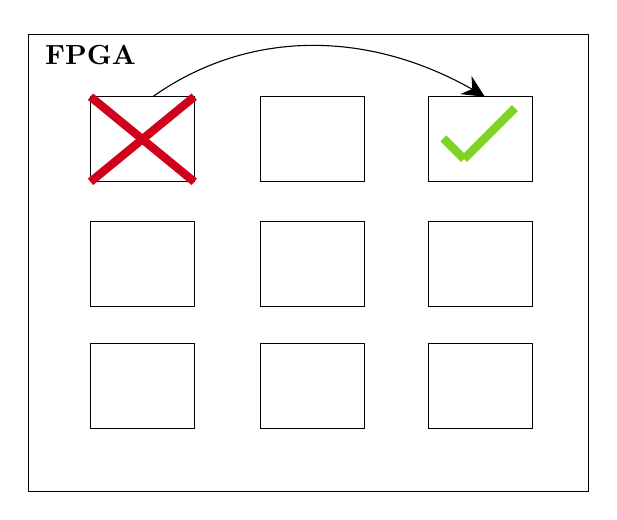
\begin{tikzpicture}[x=0.75pt,y=0.75pt,yscale=-1,xscale=1]
%uncomment if require: \path (0,279); %set diagram left start at 0, and has height of 279

%Shape: Rectangle [id:dp5787797491333819] 
\draw   (6,20) -- (276,20) -- (276,240) -- (6,240) -- cycle ;
%Shape: Rectangle [id:dp17505095690594463] 
\draw   (36,50) -- (86,50) -- (86,91) -- (36,91) -- cycle ;
%Shape: Rectangle [id:dp3058047377979807] 
\draw   (36,110) -- (86,110) -- (86,151) -- (36,151) -- cycle ;
%Shape: Rectangle [id:dp004684645465554249] 
\draw   (36,169) -- (86,169) -- (86,210) -- (36,210) -- cycle ;
%Shape: Rectangle [id:dp3077757040785931] 
\draw   (118,50) -- (168,50) -- (168,91) -- (118,91) -- cycle ;
%Shape: Rectangle [id:dp7450799349257811] 
\draw   (118,110) -- (168,110) -- (168,151) -- (118,151) -- cycle ;
%Shape: Rectangle [id:dp2725857150503048] 
\draw   (118,169) -- (168,169) -- (168,210) -- (118,210) -- cycle ;
%Shape: Rectangle [id:dp3816815123242099] 
\draw   (199,50) -- (249,50) -- (249,91) -- (199,91) -- cycle ;
%Shape: Rectangle [id:dp2885393682660524] 
\draw   (199,110) -- (249,110) -- (249,151) -- (199,151) -- cycle ;
%Shape: Rectangle [id:dp4969175268738504] 
\draw   (199,169) -- (249,169) -- (249,210) -- (199,210) -- cycle ;
%Straight Lines [id:da8580754234796655] 
\draw [color={rgb, 255:red, 208; green, 2; blue, 27 }  ,draw opacity=1 ][line width=3]    (36,50) -- (86,91) ;


%Straight Lines [id:da5772916268060835] 
\draw [color={rgb, 255:red, 208; green, 2; blue, 27 }  ,draw opacity=1 ][line width=3]    (86,50) -- (36,91) ;


%Curve Lines [id:da5702734861080319] 
\draw    (66,50) .. controls (112.04,17.33) and (171.3,17) .. (224.39,49.02) ;
\draw [shift={(226,50)}, rotate = 211.67000000000002] [fill={rgb, 255:red, 0; green, 0; blue, 0 }  ][line width=0.75]  [draw opacity=0] (10.72,-5.15) -- (0,0) -- (10.72,5.15) -- (7.12,0) -- cycle    ;

%Straight Lines [id:da7282259837027933] 
\draw [color={rgb, 255:red, 126; green, 211; blue, 33 }  ,draw opacity=1 ][line width=3]    (240.5,55.5) -- (216,80) ;


%Straight Lines [id:da7142424530641487] 
\draw [color={rgb, 255:red, 126; green, 211; blue, 33 }  ,draw opacity=1 ][line width=3]    (216,80) -- (206,70) ;



% Text Node
\draw (36,30) node  [align=left] {\textbf{FPGA}};


\end{tikzpicture}
}
    \caption{Internal Fault Mitigation - functionality from a faulty tile is moved to a healthy area with \gls{DPR}}\label{fig:internalFaultMitigation}
\end{figure}
%\tikzset{every picture/.style={line width=0.25pt}} %set default line width to 0.75pt        

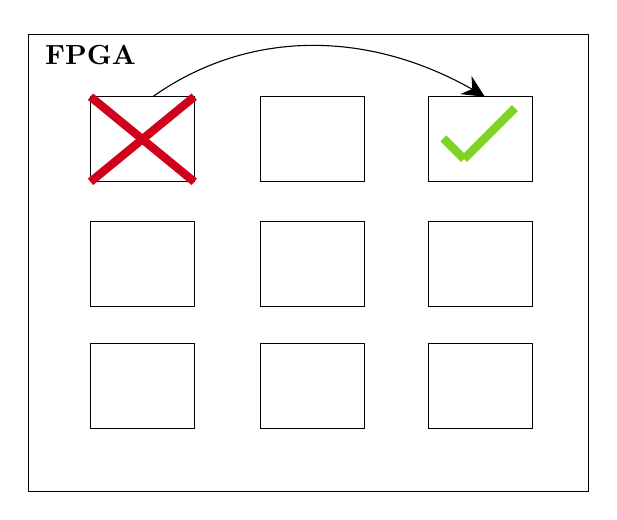
\begin{tikzpicture}[x=0.75pt,y=0.75pt,yscale=-1,xscale=1]
%uncomment if require: \path (0,279); %set diagram left start at 0, and has height of 279

%Shape: Rectangle [id:dp5787797491333819] 
\draw   (6,20) -- (276,20) -- (276,240) -- (6,240) -- cycle ;
%Shape: Rectangle [id:dp17505095690594463] 
\draw   (36,50) -- (86,50) -- (86,91) -- (36,91) -- cycle ;
%Shape: Rectangle [id:dp3058047377979807] 
\draw   (36,110) -- (86,110) -- (86,151) -- (36,151) -- cycle ;
%Shape: Rectangle [id:dp004684645465554249] 
\draw   (36,169) -- (86,169) -- (86,210) -- (36,210) -- cycle ;
%Shape: Rectangle [id:dp3077757040785931] 
\draw   (118,50) -- (168,50) -- (168,91) -- (118,91) -- cycle ;
%Shape: Rectangle [id:dp7450799349257811] 
\draw   (118,110) -- (168,110) -- (168,151) -- (118,151) -- cycle ;
%Shape: Rectangle [id:dp2725857150503048] 
\draw   (118,169) -- (168,169) -- (168,210) -- (118,210) -- cycle ;
%Shape: Rectangle [id:dp3816815123242099] 
\draw   (199,50) -- (249,50) -- (249,91) -- (199,91) -- cycle ;
%Shape: Rectangle [id:dp2885393682660524] 
\draw   (199,110) -- (249,110) -- (249,151) -- (199,151) -- cycle ;
%Shape: Rectangle [id:dp4969175268738504] 
\draw   (199,169) -- (249,169) -- (249,210) -- (199,210) -- cycle ;
%Straight Lines [id:da8580754234796655] 
\draw [color={rgb, 255:red, 208; green, 2; blue, 27 }  ,draw opacity=1 ][line width=3]    (36,50) -- (86,91) ;


%Straight Lines [id:da5772916268060835] 
\draw [color={rgb, 255:red, 208; green, 2; blue, 27 }  ,draw opacity=1 ][line width=3]    (86,50) -- (36,91) ;


%Curve Lines [id:da5702734861080319] 
\draw    (66,50) .. controls (112.04,17.33) and (171.3,17) .. (224.39,49.02) ;
\draw [shift={(226,50)}, rotate = 211.67000000000002] [fill={rgb, 255:red, 0; green, 0; blue, 0 }  ][line width=0.75]  [draw opacity=0] (10.72,-5.15) -- (0,0) -- (10.72,5.15) -- (7.12,0) -- cycle    ;

%Straight Lines [id:da7282259837027933] 
\draw [color={rgb, 255:red, 126; green, 211; blue, 33 }  ,draw opacity=1 ][line width=3]    (240.5,55.5) -- (216,80) ;


%Straight Lines [id:da7142424530641487] 
\draw [color={rgb, 255:red, 126; green, 211; blue, 33 }  ,draw opacity=1 ][line width=3]    (216,80) -- (206,70) ;



% Text Node
\draw (36,30) node  [align=left] {\textbf{FPGA}};


\end{tikzpicture}

\glspl{FPGA} provide high flexibility and good performance in many areas that require a high amount of concurrent computing and therefore benefit from a dedicated hardware implementation.
These properties prove useful for applications in the domain of aerospace and help to reduce the cost for satellites and spacecraft while providing a high flexibility. 
But \glspl{FPGA} are especially vulnerable to cosmic radiation which can create a multitude of internal errors in the \gls{FPGA} and thereby breaking its intended functionality \cite{ito_total_2015}.
While there are radiation hardened \glspl{FPGA} available on the market, the mass of a space embedded system is still composed of 80\% radiation shielding.
This shielding is still not able to provide a perfect protection from radiation.
Therefore, solutions for fault mitigation in aerospace \glspl{FPGA} need to be developed on the architectural level instead of the physical level. 
This may also provide the advantage of lower requirements for radiation shielding and therefore a reduced cost for payload on rocket launches.

\subsection{Types of Internal Faults}
There are different types of faults that may occur in the lifetime of an \gls{FPGA}, a short overview over the most relevant ones is given in the following.
\par
\textbf{Transient Faults}
\begin{itemize}
    \item \glspl{SEU}, e.g. radiation induced \cite{alkady_fault-tolerant_2014}, \cite{lee_fault-tolerant_2017}
    \begin{itemize}
    \item Change of logic state in memory cell
    \item Commonly tackled by redundancy
    \item Built-in fault detection unit possible
    \end{itemize}
    \item Single Bit Errors (SBEs)
    \item Single Event Transients (SETs)
    \item Address Decoding Faults
\end{itemize}

Faults occur either in the interconnect of the \gls{FPGA} (which uses up to 80\% of the available silicon) or in its actual logic blocks \cite{alkady_fault-tolerant_2014}, \cite{jing_huang_routability_2004}.
\par
\textbf{Permanent Faults}
\begin{itemize}
    \item Time Dependant Dielectric Breakdowns (TDDBs)
    \item Electro Migration
    \item Hot Carrier Effect
\end{itemize}
\subsection{Mitigation Strategies for Internal Faults}
To mitigate the aforementioned internal faults in an \gls{FPGA}, different strategies can be employed.
This section is going to introduce the most common concepts and how they can be combined.


\section{\gls{DPR} for External Fault Mitigation}\label{ExternalFaults}
Redundancy is a necessary feature to increase the dependability of a system.
Systems that have a need for high dependability encompass e.g. any safety critical system where a fault can result in the harm or even loss of human live.
Systems where maintenance may be difficult or expensive are another set of examples where redundancy is useful.
Redundancy can be achieved through the provision of multiple hardware entities that perform the same task.
If one hardware entity fails, another can take over and supply the expected functionality.
This can get expensive when there are multiple smaller hardware entities that perform specific computational work. 
To reduce space usage and cost, a general purpose \gls{CPU} can be used.
This \gls{CPU} can then emulate the functionality of the faulty hardware and thereby mitigates the fault. 
But this approach introduces new margin for error, as a two-pronged development may lead to discrepancies.
Another issue are real-time requirements that need to be fulfilled.
A regular \gls{CPU} may not be able to provide concurrent computations or the required performance, as the emulated hardware (or software) may be too complex.

A solution to these problems is the usage of \glspl{FPGA} as a means of redundancy. 
As the \gls{FPGA} can be reconfigured with different functionality during runtime, it reduces the total amount of hardware that is needed to achieve redundancy.
Unlike \glspl{CPU}, \glspl{FPGA} provide better means for concurrent computation and are suitable to emulate multiple faulty hardware entities in a more appropriate manner. %TODO: Citation needed

\begin{figure}
    \resizebox{\columnwidth}{!}{

\tikzset{every picture/.style={line width=0.75pt}} %set default line width to 0.75pt        

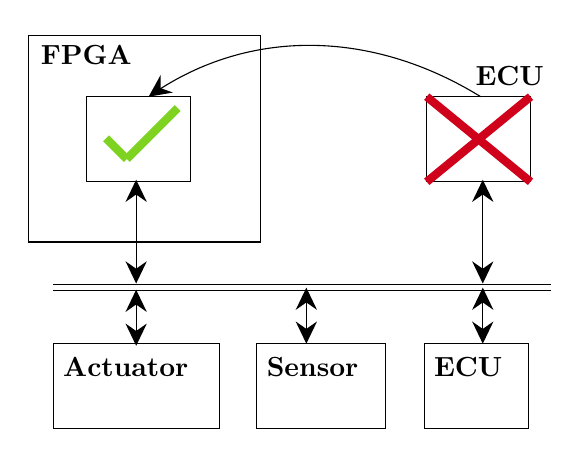
\begin{tikzpicture}[x=0.75pt,y=0.75pt,yscale=-1,xscale=1]
%uncomment if require: \path (0,279); %set diagram left start at 0, and has height of 279

%Shape: Rectangle [id:dp5787797491333819] 
\draw   (8,20.5) -- (120,20.5) -- (120,120) -- (8,120) -- cycle ;
%Shape: Rectangle [id:dp17505095690594463] 
\draw   (36,50) -- (86,50) -- (86,91) -- (36,91) -- cycle ;
%Shape: Rectangle [id:dp004684645465554249] 
\draw   (20,169) -- (100,169) -- (100,210) -- (20,210) -- cycle ;
%Shape: Rectangle [id:dp2725857150503048] 
\draw   (118,169) -- (180,169) -- (180,210) -- (118,210) -- cycle ;
%Shape: Rectangle [id:dp2885393682660524] 
\draw   (200,50) -- (250,50) -- (250,91) -- (200,91) -- cycle ;
%Shape: Rectangle [id:dp4969175268738504] 
\draw   (199,169) -- (249,169) -- (249,210) -- (199,210) -- cycle ;
%Straight Lines [id:da8580754234796655] 
\draw [color={rgb, 255:red, 208; green, 2; blue, 27 }  ,draw opacity=1 ][line width=3]    (200,50) -- (250,91) ;


%Straight Lines [id:da5772916268060835] 
\draw [color={rgb, 255:red, 208; green, 2; blue, 27 }  ,draw opacity=1 ][line width=3]    (250,50) -- (200,91) ;


%Curve Lines [id:da5702734861080319] 
\draw    (68.1,48.54) .. controls (114.3,17.01) and (173.3,17.5) .. (226,50) ;

\draw [shift={(66,50)}, rotate = 324.64] [fill={rgb, 255:red, 0; green, 0; blue, 0 }  ][line width=0.75]  [draw opacity=0] (10.72,-5.15) -- (0,0) -- (10.72,5.15) -- (7.12,0) -- cycle    ;
%Straight Lines [id:da7282259837027933] 
\draw [color={rgb, 255:red, 126; green, 211; blue, 33 }  ,draw opacity=1 ][line width=3]    (80,55.5) -- (55.5,80) ;


%Straight Lines [id:da7142424530641487] 
\draw [color={rgb, 255:red, 126; green, 211; blue, 33 }  ,draw opacity=1 ][line width=3]    (55.5,80) -- (45.5,70) ;


%Straight Lines [id:da36465994520752654] 
\draw    (20,140.5) -- (260,140.5)(20,143.5) -- (260,143.5) ;


%Straight Lines [id:da9447465253235761] 
\draw    (227,92) -- (227,138) ;
\draw [shift={(227,140)}, rotate = 270] [fill={rgb, 255:red, 0; green, 0; blue, 0 }  ][line width=0.75]  [draw opacity=0] (10.72,-5.15) -- (0,0) -- (10.72,5.15) -- (7.12,0) -- cycle    ;
\draw [shift={(227,90)}, rotate = 90] [fill={rgb, 255:red, 0; green, 0; blue, 0 }  ][line width=0.75]  [draw opacity=0] (10.72,-5.15) -- (0,0) -- (10.72,5.15) -- (7.12,0) -- cycle    ;
%Straight Lines [id:da358175601755349] 
\draw    (60,92) -- (60,138) ;
\draw [shift={(60,140)}, rotate = 270] [fill={rgb, 255:red, 0; green, 0; blue, 0 }  ][line width=0.75]  [draw opacity=0] (10.72,-5.15) -- (0,0) -- (10.72,5.15) -- (7.12,0) -- cycle    ;
\draw [shift={(60,90)}, rotate = 90] [fill={rgb, 255:red, 0; green, 0; blue, 0 }  ][line width=0.75]  [draw opacity=0] (10.72,-5.15) -- (0,0) -- (10.72,5.15) -- (7.12,0) -- cycle    ;
%Straight Lines [id:da07393951188629155] 
\draw    (60,145) -- (60,168) ;
\draw [shift={(60,170)}, rotate = 270] [fill={rgb, 255:red, 0; green, 0; blue, 0 }  ][line width=0.75]  [draw opacity=0] (10.72,-5.15) -- (0,0) -- (10.72,5.15) -- (7.12,0) -- cycle    ;
\draw [shift={(60,143)}, rotate = 90] [fill={rgb, 255:red, 0; green, 0; blue, 0 }  ][line width=0.75]  [draw opacity=0] (10.72,-5.15) -- (0,0) -- (10.72,5.15) -- (7.12,0) -- cycle    ;
%Straight Lines [id:da8542656416019287] 
\draw    (142,144) -- (142,167) ;
\draw [shift={(142,169)}, rotate = 270] [fill={rgb, 255:red, 0; green, 0; blue, 0 }  ][line width=0.75]  [draw opacity=0] (10.72,-5.15) -- (0,0) -- (10.72,5.15) -- (7.12,0) -- cycle    ;
\draw [shift={(142,142)}, rotate = 90] [fill={rgb, 255:red, 0; green, 0; blue, 0 }  ][line width=0.75]  [draw opacity=0] (10.72,-5.15) -- (0,0) -- (10.72,5.15) -- (7.12,0) -- cycle    ;
%Straight Lines [id:da22998818326497883] 
\draw    (227,144) -- (227,167) ;
\draw [shift={(227,169)}, rotate = 270] [fill={rgb, 255:red, 0; green, 0; blue, 0 }  ][line width=0.75]  [draw opacity=0] (10.72,-5.15) -- (0,0) -- (10.72,5.15) -- (7.12,0) -- cycle    ;
\draw [shift={(227,142)}, rotate = 90] [fill={rgb, 255:red, 0; green, 0; blue, 0 }  ][line width=0.75]  [draw opacity=0] (10.72,-5.15) -- (0,0) -- (10.72,5.15) -- (7.12,0) -- cycle    ;

% Text Node
\draw (36,30) node  [align=left] {\textbf{FPGA}};
% Text Node
\draw (240,40) node  [align=left] {\textbf{ECU}};
% Text Node
\draw (220,180) node  [align=left] {\textbf{ECU}};
% Text Node
\draw (145,180) node  [align=left] {\textbf{Sensor}};
% Text Node
\draw (55,180) node  [align=left] {\textbf{Actuator}};


\end{tikzpicture}
}
    \caption{External Fault Mitigation - functionality from a faulty \gls{ECU} is provided by a module (instantiated with \gls{DPR}) within the \gls{FPGA}}\label{fig:externalFaultMitigation}
\end{figure}

\subsection{Types of External Faults}
\subsection{Mitigation Strategies for External Faults}

\section{Mitigation of Faults}
\subsection{Network on Chip - make fault-tolerant per design}
\cite{yesil_fpga_2016} adds additional network resources to a non-fault-tolerant design to mitigate interconnect faults.

\cite{lu_fault-tolerant_2015} provides a case study on implementing a fault-tolerant routing algorithm and its monitoring mechanism.
\subsection{Redundancy by need based replication}
\cite{glein_self-adaptive_2014} tackles the problem of radiation by the creation of redundant modules - based on currently measured \glspl{SEU} rates in on-chip memories.
\subsection{Dynamic Partial Self-Reconfiguration}
\cite{alkady_dynamic_2015} goes on to propose system recovery by re-instantiating defective modules into the Partially Reconfigurable block.

\cite{shanker_enhancing_nodate} proposes a similar solution in the context of \glspl{ECU}.

\cite{sharma_run-time_2018} shows an approach on how to decide which configuration is currently desired in a multi-modal / multi-task \gls{SoPC}.
\printglossaries 

\bibliographystyle{IEEEtran}
\bibliography{IEEEabrv,SocSeminar}

\end{document}
